\chapter{Our solution} \label{our:solution}


% uvod, co je v kapitole, nejdriv...
% obecne algorithmus bez rozzepsaneho gpcka

% Prvni cats - GPcko (zakodovani, init, operat., fitness jak se pocita (ale vic dole),...
% Druha - Sklearn strana, eval, samples,...

% Posledni- implementace, deap,...

% experimenty 4

In our solution we design an AutoML system for workflow optimization based on
developmental genetic programming. Compared to existing systems it supports 
arbitrary-sized pipelines as well as complex ensemble structures. We first
present in what way we use the genetic programming, then we describe the
pipeline evaluation process.

\section{Evolutionary optimization of pipelines}
The algorithm corresponds to the schema of a general genetic algorithm
\ref{alg:EA}. In this section we describe the necessary components of the
algorithm.

\subsection{Individual encoding}
The individual encoding is one of the most important parts of this system. With
ensembles and complex feature preprocessing methods like stacking or feature
union, most of the pipelines become in fact directed acyclic graphs (figure 
\ref{pic02:pipeline}). Therefore, we cannot directly use the simple tree-based
encoding. Instead we use the developmental GP with cellular encoding described
in section \ref{devGP}.
\begin{figure}[ht]\centering
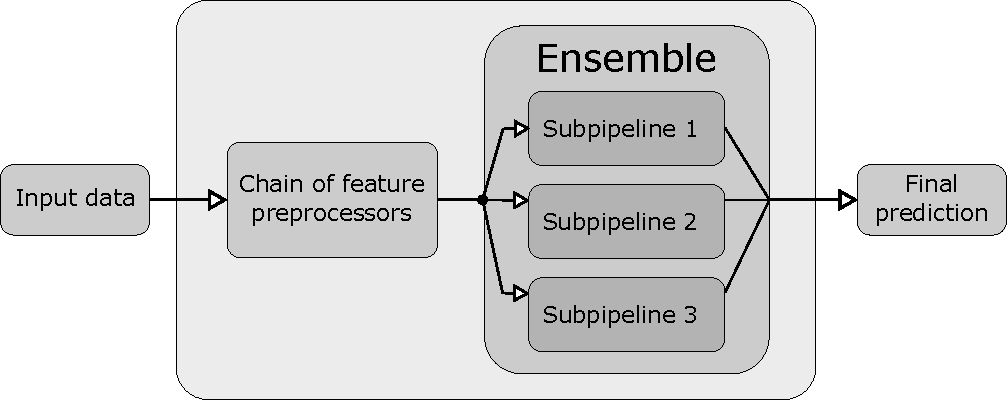
\includegraphics[width=0.8\textwidth]{../img/pipeline-pdfa.pdf}
\caption{Schema of an example pipeline}
\label{pic02:pipeline}
\end{figure}

In our case, the embryo is an empty pipeline. To create a complex pipeline, we
modify it by inserting steps into it. The process can be demonstrated on figure
\ref{pic:pipeencoding}. The root of the tree represents the embryo which will
be modified by subsequent operations. In this case, the left subtree modifies
the ensemble structure whereas the right subtree modifies the feature
preprocessor chain. The pipeline contains only one preprocessor, hence the
right subtree is terminated by the corresponding node. The left son can be
either an ensemble or a simple method. Here it is the AdaBoost ensemble which
has one base classifier. The subestimator is again a pipeline, which is composed
of a MinMaxScaler and Stochastic gradient descent classifier.

\begin{figure}[h]\centering
    \subfloat[Tree encoding]{{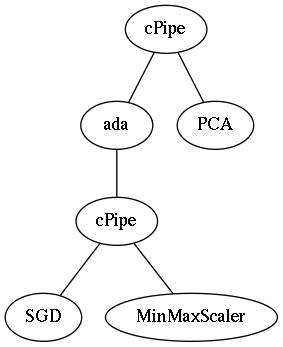
\includegraphics[width=0.3\textwidth]{../img/ada.png} }}%
    \qquad
    \subfloat[Encoded pipeline]{{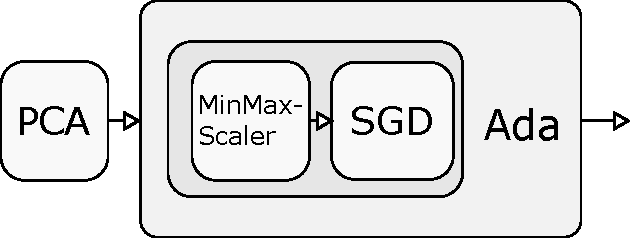
\includegraphics[width=0.6\textwidth]{../img/ada-pdfa.pdf} }}%
    \caption{An example pipeline encoded to a tree individual}%
    \label{pic:pipeencoding}%
\end{figure}

% TODO should I describe node types?
\begin{table}[b!]

\centering
%%% Tabulka používá následující balíčky:
%%%   - booktabs (\toprule, \midrule, \bottomrule)
%%%   - dcolumn (typ sloupce D: vycentrovaná čísla zarovnaná na
%%%     desetinnou čárku
%%%     Všimněte si, že ve zdrojovém kódu jsou desetinné tečky, ale
%%%     tisknou se čárky.
%%% Dále používáme příkazy \pulrad a \mc definované v makra.tex
\begin{tabular}{l l}
\toprule
\mc{\textbf{Node identifier}} & \mc{\textbf{Operation}} \\
\midrule
cPipe & Create pipeline with a preprocessor chain and a predictor \\
cPred & Create pipeline only with a predictor \\
cData & Create preprocessor chain with feature selector and scaler \\
cFeatSelect & Create preprocessor chain only with a feature selector \\
cScale & Create preprocessor chain only with a scaler \\
dUnion & Create feature union in the preprocessor chain \\
\textit{classifier id} & Insert classifier \\
\textit{ensemble id} & Insert ensemble \\
\textit{preprocessor id} & Insert preprocessor \\
\bottomrule

\end{tabular}
\caption{Nodes representing modifying operations}\label{tab03:nodes}

\end{table}

\subsection{Genetic operators}

\subsection{Fitness and selection}

\section{Evaluation and performance estimation}

\section{Implementation}